%==============================================================================
% Sjabloon poster bachproef
%==============================================================================
% Gebaseerd op document class `a0poster' door Gerlinde Kettl en Matthias Weiser
% Aangepast voor gebruik aan HOGENT door Jens Buysse en Bert Van Vreckem

\documentclass[a0,portrait]{hogent-poster}

% Extra packages voor diagram
\usepackage{tikz}
\usetikzlibrary{shapes.geometric, arrows.meta, positioning, shadows}

% Definieer kleuren (indien niet in template)
\definecolor{primarygreen}{RGB}{30, 100, 50}
\definecolor{lightgreen}{RGB}{200, 230, 200}
\definecolor{primaryblue}{RGB}{40, 80, 150}
\definecolor{lightblue}{RGB}{200, 220, 240}

% Minder ruimte tussen items
\setlength{\itemsep}{0pt}
\setlength{\parskip}{0pt}

% Info over de opleiding
\course{Graduaatsproef}
\studyprogramme{Graduaat in het Programmeren}
\academicyear{2025-2026}
\institution{Hogeschool Gent, Valentin Vaerwyckweg 1, 9000 Gent}

% Info over de bachelorproef
\title{AI-gestuurd Callcenter voor Tandartspraktijken}
\subtitle{Automatisering van patiëntcommunicatie met Twilio en OpenAI}
\author{Abdil Mavzer}
\email{abdil.mavzer@student.hogent.be}
\supervisor{Luc Vervoort}
\cosupervisor{Jona Decubber (TurnUp)}
\projectrepo{https://github.com/Abdilz/Mavzer_Abdil_GraduaatsProef-2025-2026.git}

% Indien ingevuld, wordt deze informatie toegevoegd aan het einde van de
% abstract. Zet in commentaar als je dit niet wilt.
\specialisation{Programmeren}
\keywords{OpenAI, Twilio, Voice AI, ASP.NET Core}
%\projectrepo{Niet publiek (bedrijfscode)}

\begin{document}

\maketitle

\begin{abstract}
Tandartspraktijken besteden dagelijks uren aan telefonisch afspraakbeheer. Dit project presenteert een AI-gestuurd callcenter dat deze taken volledig automatiseert. Door de integratie van \textbf{Twilio} (telefonie) en \textbf{OpenAI GPT} (conversatie) kunnen patiënten 24/7 in drie talen terecht voor het bekijken, annuleren en verzetten van afspraken.
\end{abstract}

\begin{multicols}{2}

\section{Probleemstelling}
Receptionisten in tandartspraktijken spenderen een aanzienlijk deel van hun tijd aan repetitieve telefoontjes:
\begin{itemize}\setlength{\itemsep}{0pt}
    \item \textbf{Beperkte bereikbaarheid}: Enkel tijdens kantooruren
    \item \textbf{Wachttijden}: Patiënten in de wachtrij tijdens piekmomenten
    \item \textbf{Taalbarrières}: Meertalige patiëntenpopulatie
    \item \textbf{Repetitief werk}: Dezelfde vragen, dag na dag
\end{itemize}
\textbf{Onderzoeksvraag:} Hoe kan spraakgestuurde AI de telefonische dienstverlening automatiseren met behoud van klanttevredenheid?

\section{Methodologie}
Het systeem werd iteratief ontwikkeld met focus op drie pijlers:

\textbf{1. Telefonie-integratie (Twilio)}
\begin{itemize}\setlength{\itemsep}{0pt}
    \item Inkomende oproepen via programmeerbare telefoonnummers
    \item Spraakherkenning met Twilio Speech-to-Text
    \item Text-to-Speech met Amazon Polly stemmen
    \item IVR-menu voor taalkeuze (NL/EN/FR)
\end{itemize}

\textbf{2. AI-conversatie (OpenAI GPT)}
\begin{itemize}\setlength{\itemsep}{0pt}
    \item Natuurlijke taalverwerking voor intentieherkenning
    \item Function calling voor gestructureerde acties
    \item Context-aware gesprekken over meerdere beurten
\end{itemize}

\textbf{3. Backend (ASP.NET Core + Azure)}
\begin{itemize}\setlength{\itemsep}{0pt}
    \item RESTful API voor praktijkintegratie
    \item Gespreksopname en transcriptie
    \item Beveiligde opslag via Azure Key Vault
\end{itemize}

\section{Systeemarchitectuur}
\begin{center}
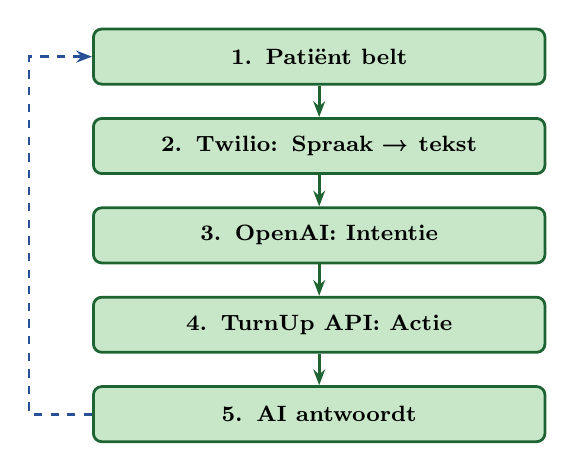
\begin{tikzpicture}[
    node distance=0.4cm,
    box/.style={rectangle, rounded corners=3pt, draw=primarygreen, line width=1pt,
                fill=lightgreen, text width=5.5cm, minimum height=0.7cm, align=center,
                font=\footnotesize\bfseries},
    arrow/.style={-{Stealth[length=2mm, width=1.5mm]}, line width=1pt, primarygreen}
]
\node[box] (patient) {1. Patiënt belt};
\node[box, below=of patient] (twilio) {2. Twilio: Spraak → tekst};
\node[box, below=of twilio] (openai) {3. OpenAI: Intentie};
\node[box, below=of openai] (api) {4. TurnUp API: Actie};
\node[box, below=of api] (response) {5. AI antwoordt};
\draw[arrow] (patient) -- (twilio);
\draw[arrow] (twilio) -- (openai);
\draw[arrow] (openai) -- (api);
\draw[arrow] (api) -- (response);
\draw[arrow, dashed, primaryblue] (response.west) -- ++(-0.8,0) |- (patient.west);
\end{tikzpicture}
\captionof{figure}{Gespreksflow}
\end{center}

\section{Implementatie}
De AI-assistent beschikt over vijf kernfuncties via OpenAI's function calling:
\begin{itemize}\setlength{\itemsep}{0pt}
    \item \texttt{lookup\_customer} -- Patiëntgegevens ophalen
    \item \texttt{cancel\_appointment} -- Afspraak annuleren
    \item \texttt{reschedule\_appointment} -- Afspraak verzetten
    \item \texttt{add\_to\_waitlist} -- Toevoegen aan wachtlijst
    \item \texttt{transfer\_to\_practice} -- Doorverbinden
\end{itemize}
Op basis van de gedetecteerde intentie kiest het AI-model automatisch de juiste functie.

\section{Resultaten}
Het systeem werd getest met echte gebruikers in productieomgeving:
\begin{itemize}\setlength{\itemsep}{0pt}
    \item \textbf{24/7 beschikbaarheid} zonder menselijke tussenkomst
    \item \textbf{Drie talen} volledig ondersteund (NL, EN, FR)
    \item \textbf{Gemiddelde gespreksduur}: minder dan 2 minuten
    \item \textbf{Volledige logging}: opname, transcriptie, uitkomst
    \item \textbf{Naadloze integratie} met bestaande praktijksoftware
\end{itemize}

\section{Leerervaringen}
Dit project heeft waardevolle technische en persoonlijke vaardigheden opgeleverd:
\begin{itemize}\setlength{\itemsep}{0pt}
    \item \textbf{Zelfstandig werken}: Volledige projectverantwoordelijkheid van analyse tot deployment
    \item \textbf{Webhooks}: Event-driven communicatie tussen Twilio en backend
    \item \textbf{WebSockets}: Real-time bidirectionele datacommunicatie
    \item \textbf{AI-tools}: Effectief inzetten van ChatGPT en Copilot voor ontwikkeling
    \item \textbf{API-integratie}: Werken met externe diensten (Twilio, OpenAI, TurnUp)
\end{itemize}

\section{Conclusie}
Dit project toont aan dat conversationele AI effectief kan worden ingezet voor klantenservice in de zorgsector. De combinatie van Twilio en OpenAI biedt een \textbf{schaalbare}, \textbf{meertalige} en \textbf{kostenefficiënte} oplossing die zowel patiënten als praktijkmedewerkers ten goede komt.

\section{Toekomstig Werk}
\begin{itemize}\setlength{\itemsep}{0pt}
    \item \textbf{WebSockets}: Overschakelen van webhooks naar WebSockets voor lagere latentie
    \item \textbf{Real-time streaming}: Conversatie tijdens spraakherkenning al verwerken
    \item \textbf{Edge cases}: Verfijnen van dialectherkenning en achtergrondgeluid
    \item \textbf{Outbound calling}: Proactieve afspraakherinneringen
    \item \textbf{RAG-integratie}: Beantwoorden van praktijkspecifieke vragen
    \item \textbf{Uitbreiding}: Huisartsen, kinesisten, andere zorgsectoren
\end{itemize}

\end{multicols}
\end{document}
